\chapter{Results}
\label{sec:results}
\section{Current results Car}

Problem:
A car with fully-observable 2D-state: [position, velocity] needs to move from 
initial position $x_0=0$\si{\metre} and initial velocity $v_0=0$\si{\metre\per\ts} to 
goal position $x_F=\SI{2.0}{\metre}$. The action taken at every time-step \si{\ts}, 
with a discretization of $t_d=0.1$, determines the car acceleration. 
The control input $a$ is constrained to range between [-1.0,1.0]\si{\metre\per\square\ts}.
Per every time-step passed before it reaches the goal, the car receives a penalization
reward $R_{\si[]{\ts}}=-10$ 
If the car reaches the goal position, it receives a reward $R_F=+270$ and the episode ends.
Otherwise, after $T_F=400$\si{\ts} the episode ends (with no extra penalization).

\subsection{Case 1: No velocity penalization}
Using both DDPG and CVAR-DDPG algorithms, the car arrives at the goal position.
Both with a maximum acceleration kept throughout the whole episode.

For this setup we have:

\begin{equation*}
    x = x_0 + v_0 \frac{\si{\ts} }{10} + 0.5a \big ( \frac{\si{\ts} }{10} \big )^2
\end{equation*}
In the optimal case, the car keeps an acceleration of $\SI{1}{\metre\per\square\ts}$ for the whole episode, and hence reaches $x_F=2$\si{\metre} with 20 time-steps.
Hence the final cumulative reward $G_T= (20+1) R_{\si{\ts} } + R_{F}=60$.

\begin{figure}[ht]
        \centering
        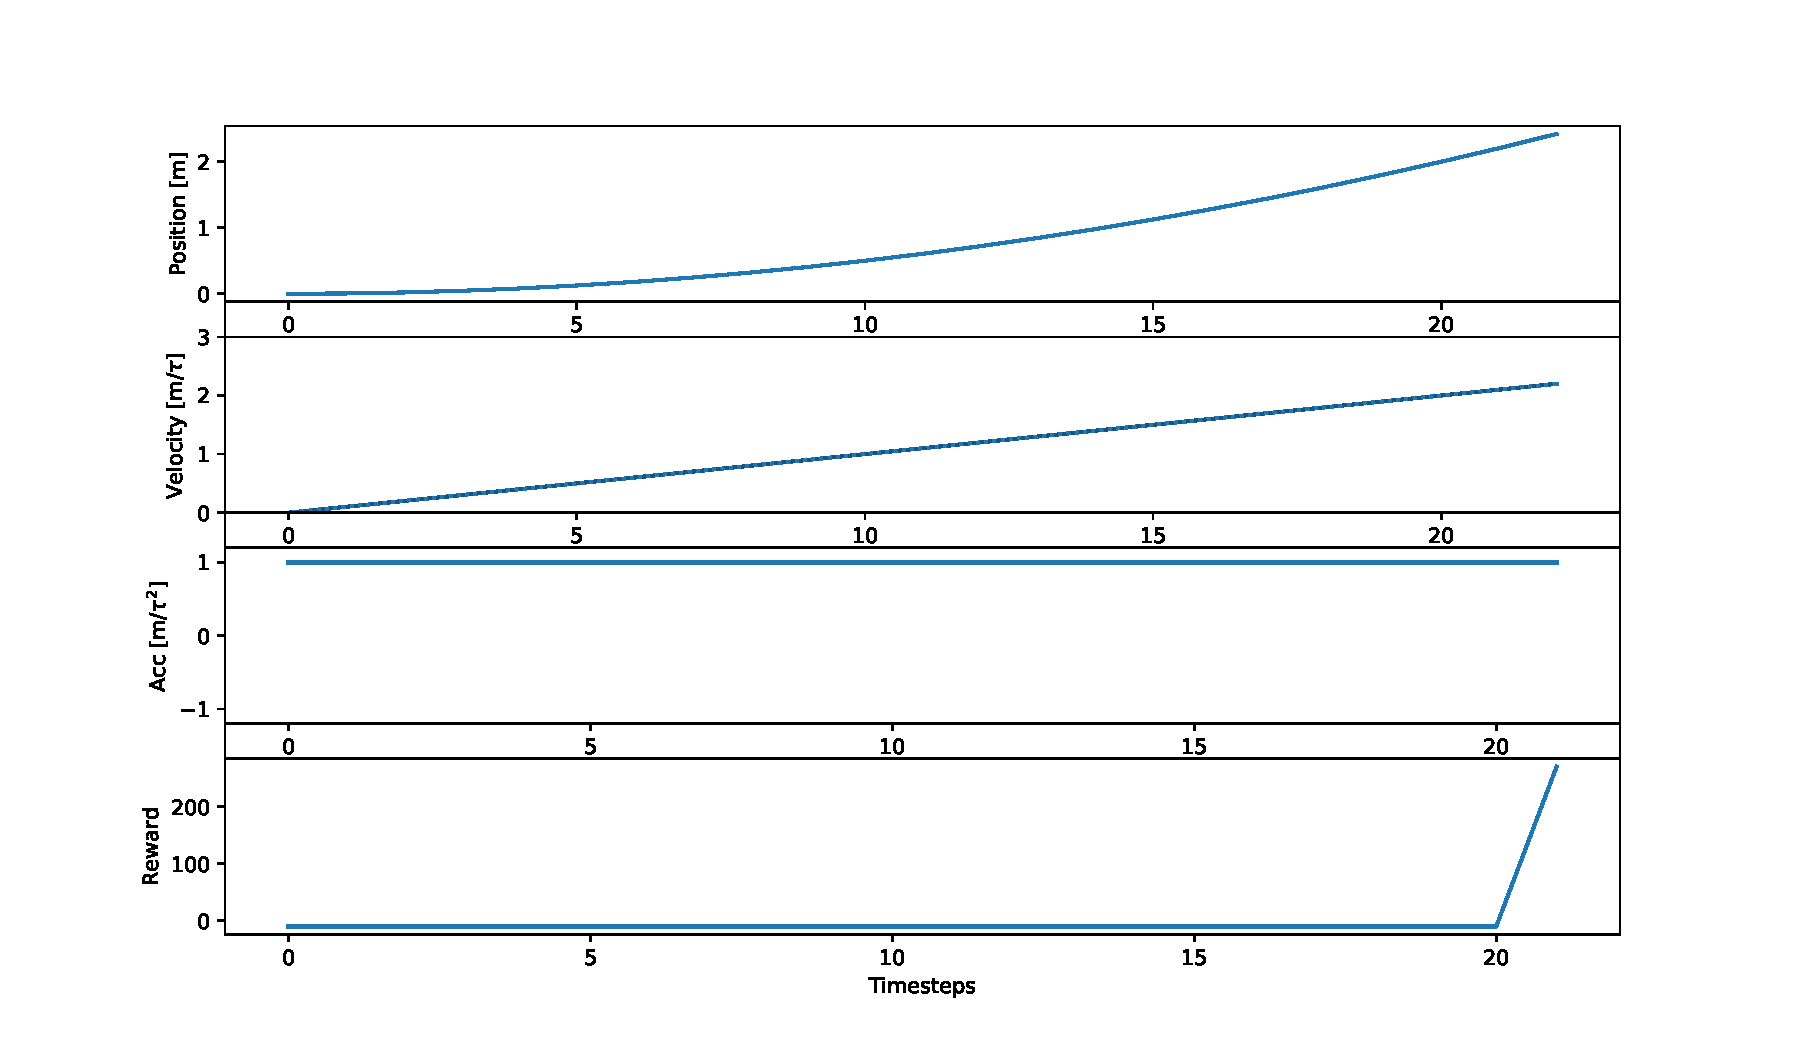
\includegraphics[width=0.8\textwidth]{images/Car/DDPG/Trajectory_DDPG_nopenal_edit.pdf}
        \caption{Car trajectory using DDPG and algorithm without velocity penalization. 
         (Same behavior for CVAR-DDPG algorithm).}
        \label{traj1_ddpg_nopenal}
    
\end{figure}

Starting from $x_0=0$\si\metre, the car reaches a velocity of 1\si{\metre\per\ts} after
10 time-steps, at $x_{\tau=10}=0.5$.
Keeping velocity 1\si{\metre\per\ts} through the rest of the episode,
it reaches the goal position after $14$ time-steps. 
Hence the final cumulative reward $G_T= (10+14+1) R_{\tau} + R_{F}=74$.
The reward values were chosen in order to make sure that,
for this Case 2 setting, driving with a velocity higher than 1\si{\metre\per\ts} never
induces higher cumulative rewards.


\subsection{Case 2: Velocity penalization with probability 1 }
The experiment is carried out to ensure the two algorithms manage to learn the new reward function when there is no uncertainty.
In this setup, when the car velocity exceeds 1\si{\metre\per\ts}, it receives a penalization of $R_v=-20$.
We expect both algorithms to perform similarly since there is no reward uncertainty.
As expected, both DDPG and CVAR-DDPG algorithms learn to accelerate with maximum value
till a velocity of 1\si{\metre\per\ts} is reached, 
and then they keep the velocity constant until the goal is reached.

Starting from $x_0=0$\si\metre, the car reaches a velocity of 1\si{\metre\per\ts} after 
10 time-steps, at $x_{\si{\ts}=10}=0.5$. Keeping velocity 1\si{\metre\per\ts} through 
the rest of the episode, it reaches the goal position after $14$ time-steps. 
Hence the final cumulative reward $G_T= (10+14+1) R_{\si{\ts} } + R_{F}=20$.
The reward values were chosen in order to make sure that, for this Case 2 setting,
driving with a velocity higher than 1\si{\metre\per\ts} never induces higher cumulative
rewards.

\textbf{For this Case 2 setting, the trained models were saved using Early stopping with \textit{maximal reward in episode evaluation} as a metric and with a patience of 100 episodes.}
The quantiles used for learning the actor for the CVAR-DDPG algorithm were sampled uniformly $\backsim\ U[0,1] $

\begin{figure}[ht]
        \centering
        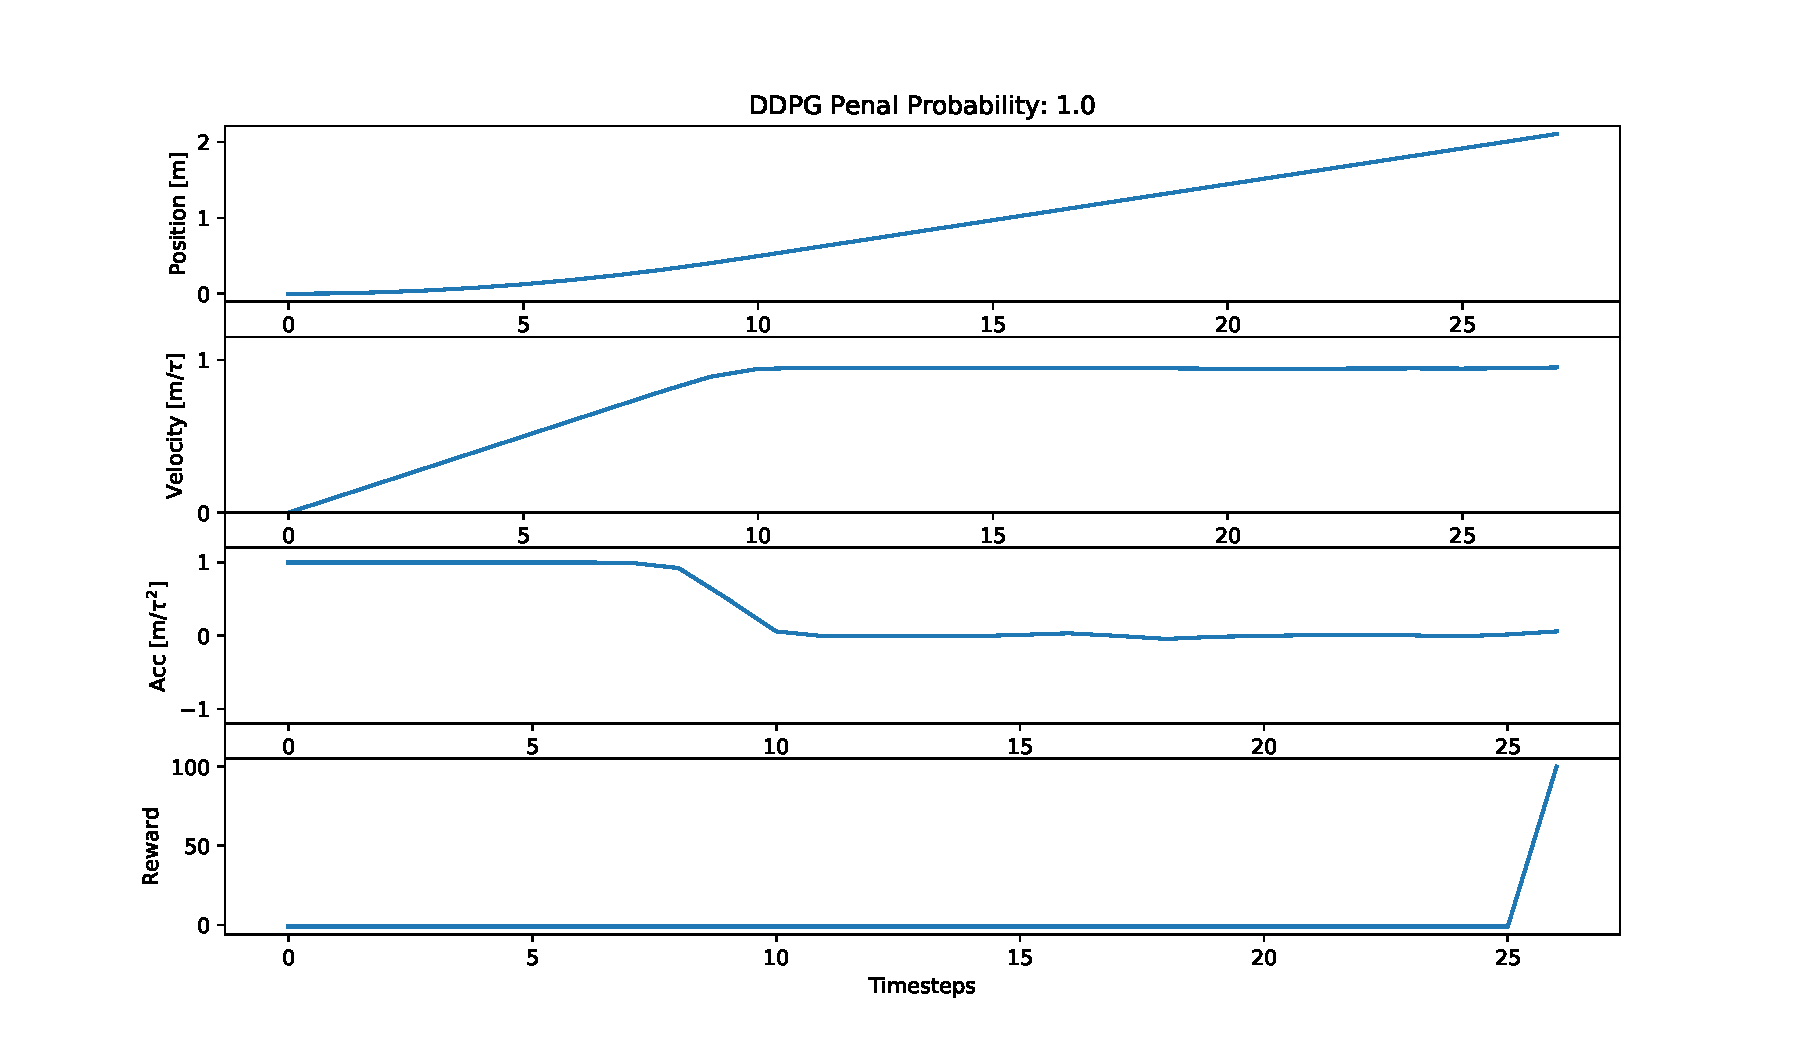
\includegraphics[width=0.8\textwidth]{images/Car/DDPG/Trajectory_DDPG_ppenal1.pdf}
        \caption{Car trajectory using DDPG algorithm and velocity penalization with probability 1 }
        \label{traj1_ddpg_probpenal1}
    
\end{figure}


\begin{figure}[ht]
        \centering
        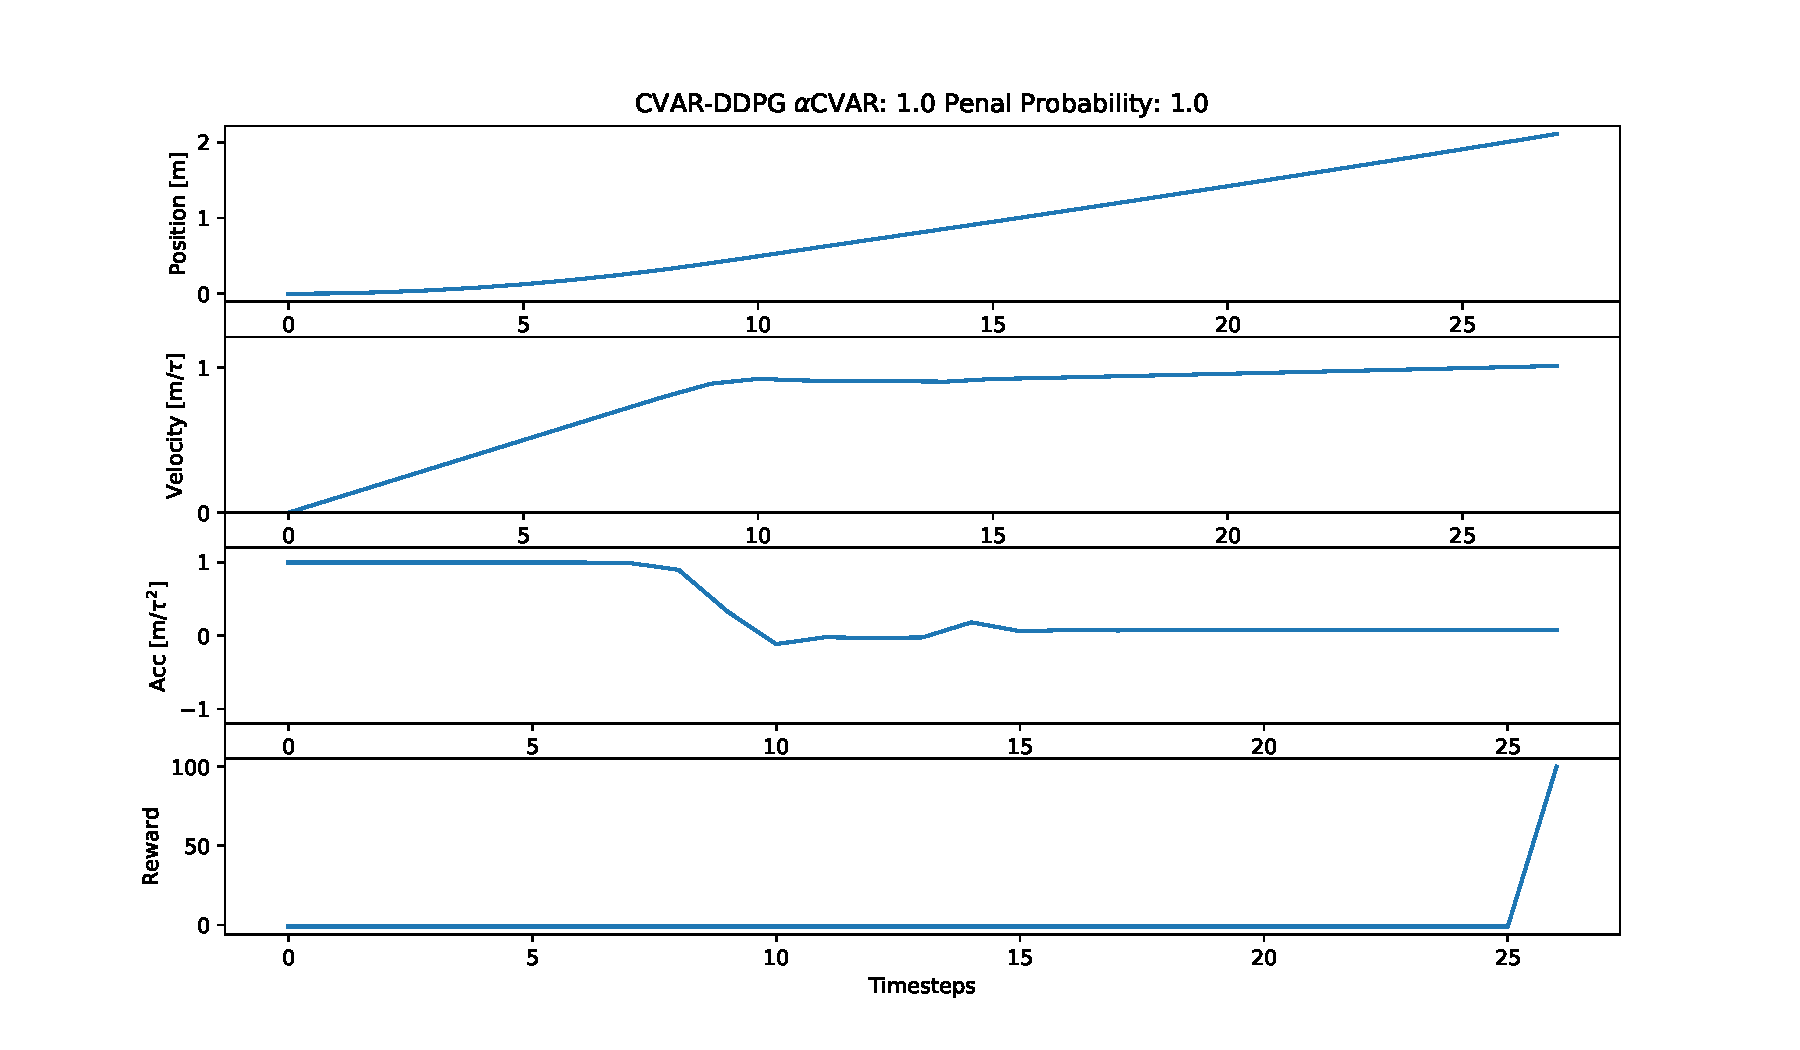
\includegraphics[width=0.8\textwidth]{images/Car/CVAR/Trajectory_CVAR_ppenal1.pdf}
        \caption{Car trajectory using CVAR-DDPG algorithm and velocity penalization with probability 1. ($\alpha$-CVAR = 1)}
        \label{traj_cvarddpg_probpenal1_cvar1}
    
\end{figure}

\newpage
\subsection{Case 3: Velocity penalization with probability P }
The experiment is carried out to show the risk-sensitiveness property of the CVAR-DDPG algorithm.

\textbf{The models saved were the ones that obtained a maximum CVAR (with a window of 
10 episodes) of the cumulative rewards during evaluation}
The quantiles used for learning the actor for the CVAR-DDPG algorithm were sampled
uniformly $\backsim\ U[0,\alpha] $ where $\alpha=0.1$


\textbf{The models saved were the ones that obtained a maximum CVAR (with a window of 
10 episodes) of the cumulative rewards during evaluation}

The quantiles used for learning the actor for the
CVAR-DDPG algorithm were sampled uniformly $\backsim\ U[0,\alpha] $ where $\alpha=0.2$.


For $P=0.2$ the CVAR-DDPG algorithm learns to saturate the velocity, even though the
probability of a penalization is low, whereas the DDPG algorithm doesn't, and keeps a
linear increase of the velocity during the whole episode.
The CVAR algorithm reaches its maximum CVAR of 64.0 at episode 220, whereas the DDPG
reaches its maximum CVAR value of 49.0 at episode 1435.

\textbf{Important issue}: Although CVAR-DDPG finds a risk-sensitive trajectory at
episode 220, it doesn't converge there and keeps oscillating and even moves towards a
risk-neutral behavior later on.
The graph in figure \ref{tail_CDF_EVOL} , shows the evolution of the sampled mean of the
tail of the sampled cumulative value distribution (CDF). (i.e. we compute via IQN the
quantile values from the tail value distribution (VD) and take the mean).
The value it converges to coincides with the maximum value of the CVAR we achieved ,but
then the actor doesn't seem to behave accordingly.


\begin{equation}
        \text{CVaR}_\alpha (Z) = \frac{1}{\alpha} \int_{0}^{\alpha} F^{-1}_Z(\tau) d\tau=\frac{1}{\alpha} \int_{0}^{\alpha} IQN(\tau) d\tau \approx 
        \frac{1}{\alpha} \frac{1}{K}\sum_{i=0}^K IQN(\tau_i) 
\end{equation}
where $\tau_i \sim U[0,\alpha]$, and IQN is the output of the IQN network for given $\tau$, representing the
value of the return for the given quantile.\\
(Values of the sampled CVAR showed in \ref{tail_CDF_EVOL} are not divided by $\alpha$ neither K )
\begin{figure}[ht]
        \centering
        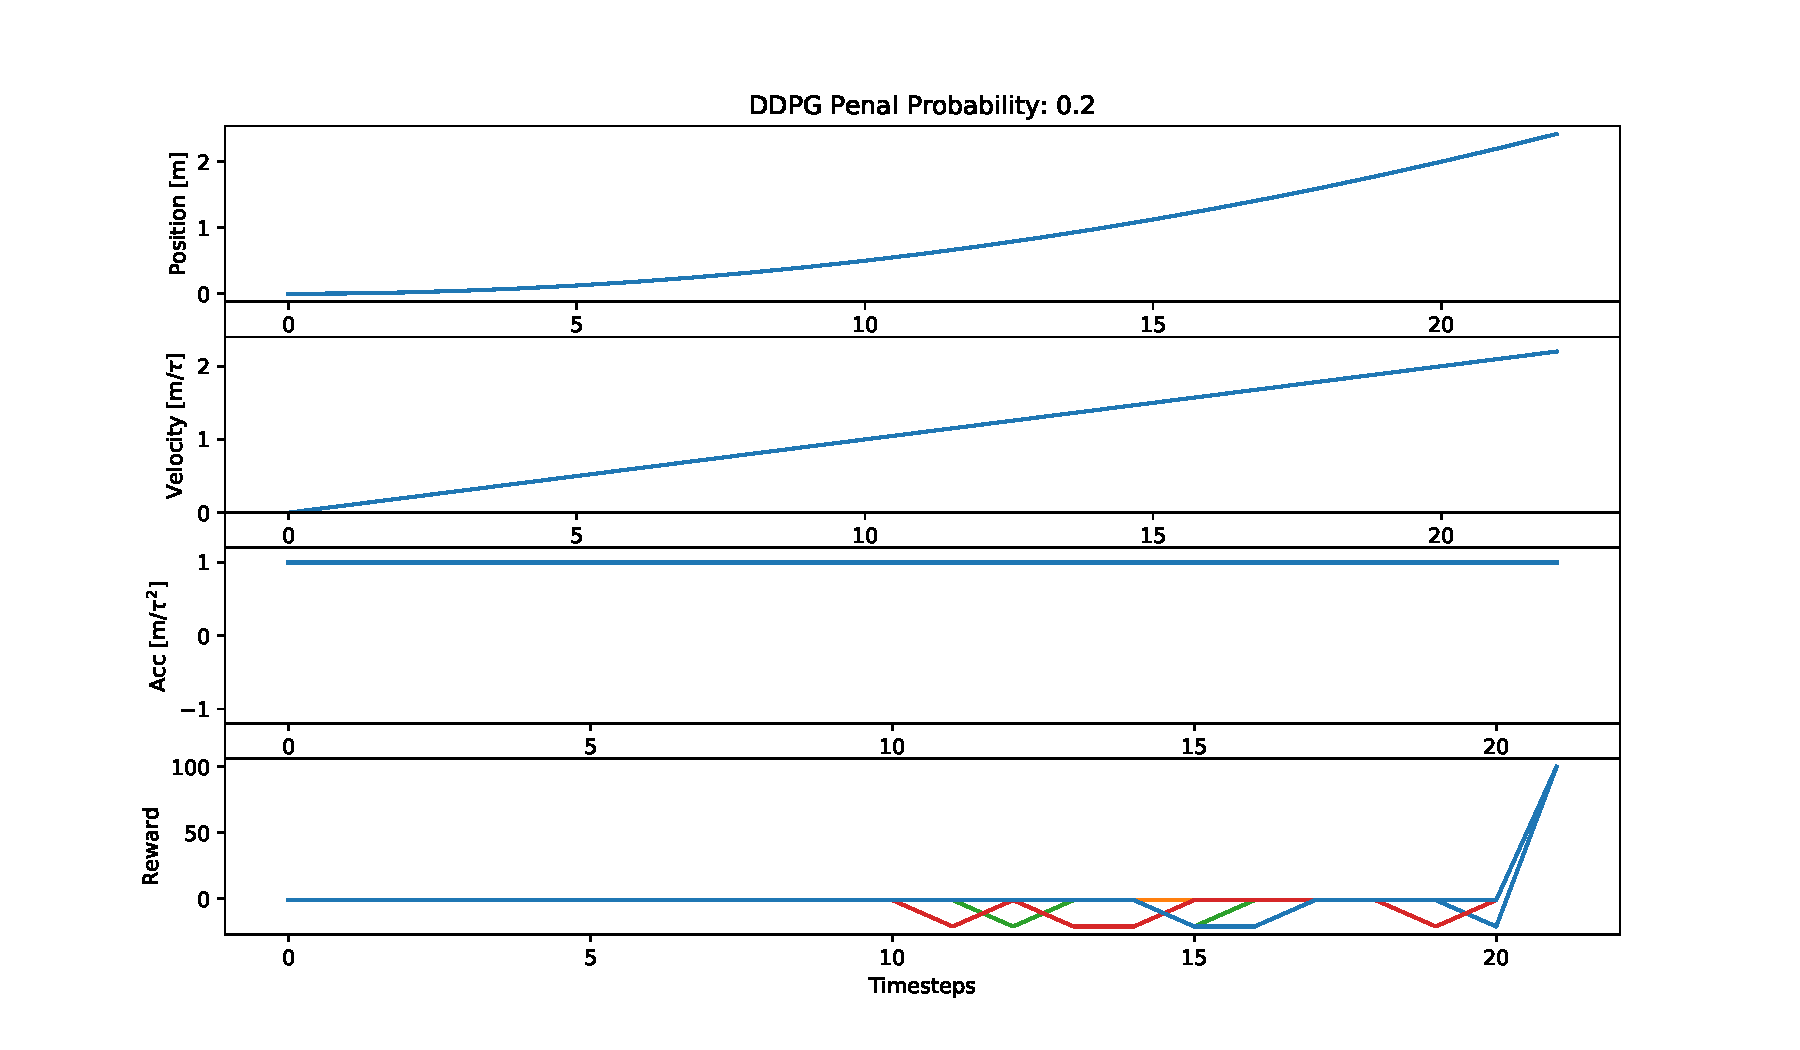
\includegraphics[width=0.8\textwidth]{images/Car/DDPG/Trajectory_DDPG_ppenal02.pdf}
        \caption{Car trajectory using DDPG algorithm and velocity penalization with
        probability P=0.2}
        \label{traj_ddpg_probpenal0.2}
    
\end{figure}

\begin{figure}[ht]
        \centering
        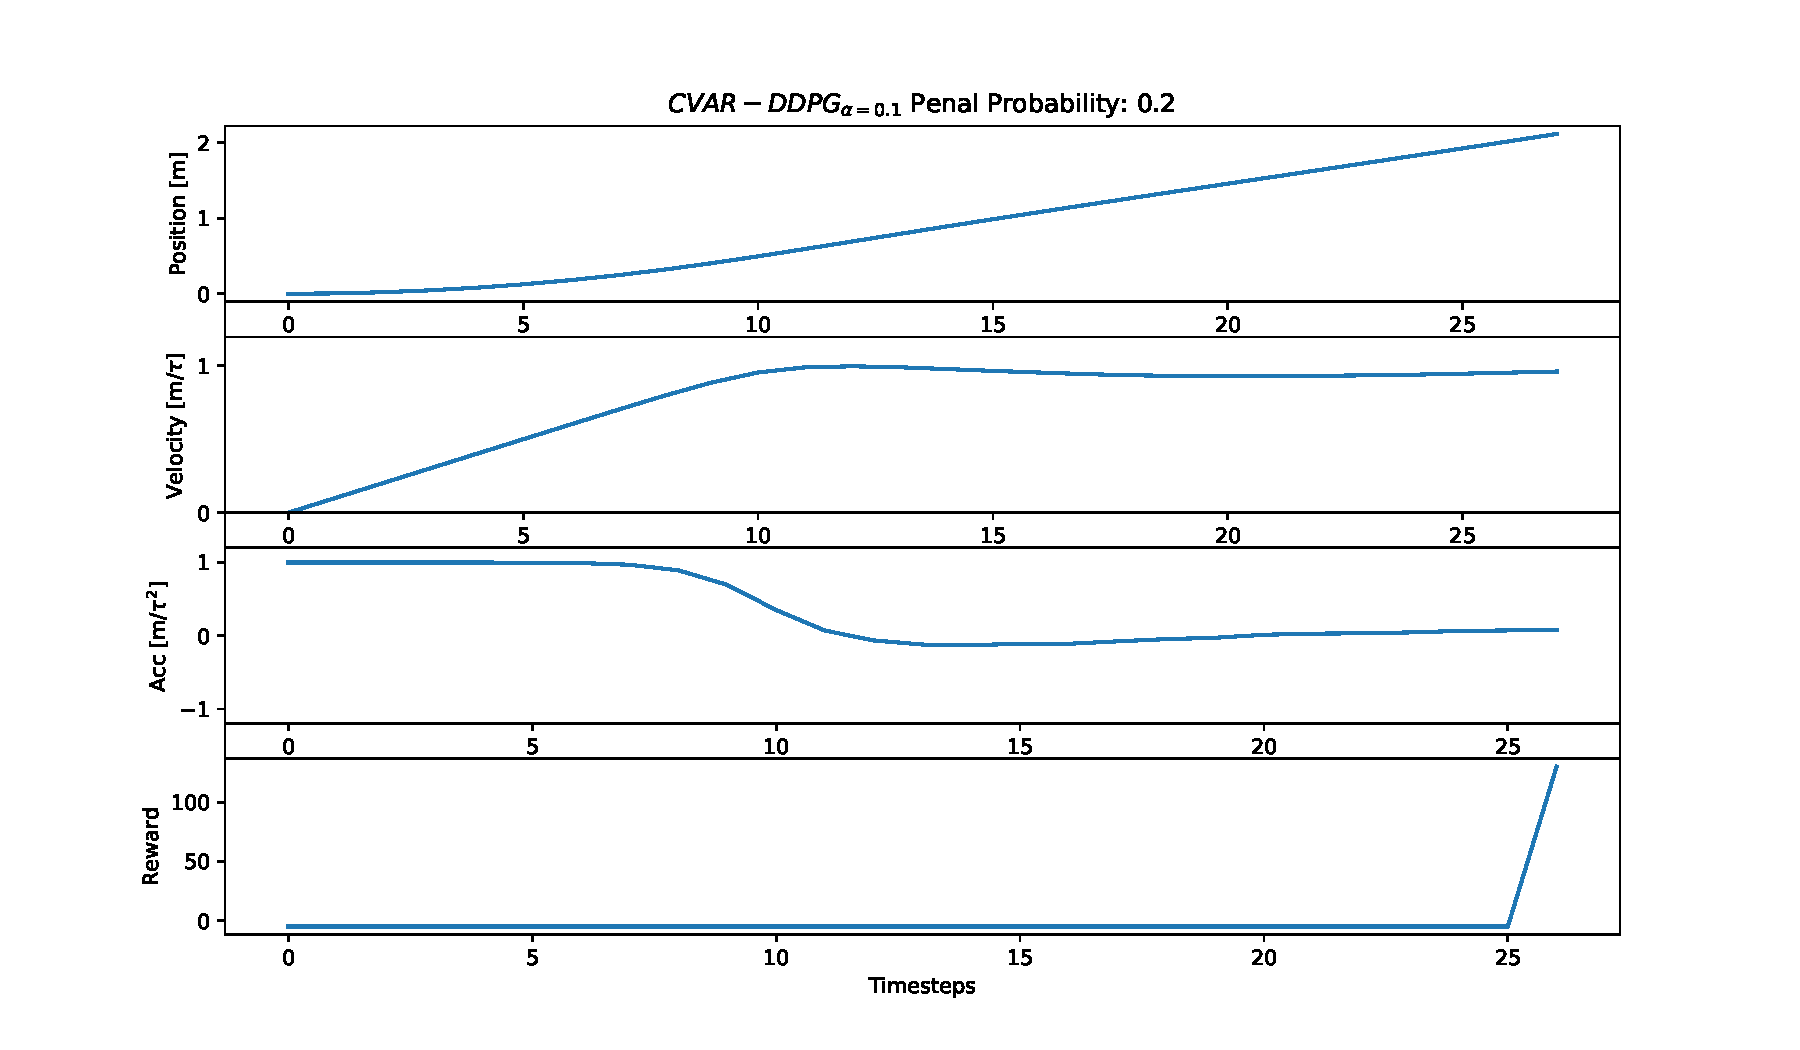
\includegraphics[width=0.8\textwidth]{images/Car/CVAR/Trajectory_CVAR_ppenal02.pdf}
        \caption{Car trajectory using CVAR-DDPG algorithm and velocity penalization with probability 0.2 and ($\alpha$-CVAR = 0.2)}
        \label{traj_cvar_ddpg_probpenal0.2_cvar0.2}
    
\end{figure}

\begin{figure}[ht]
        \centering
        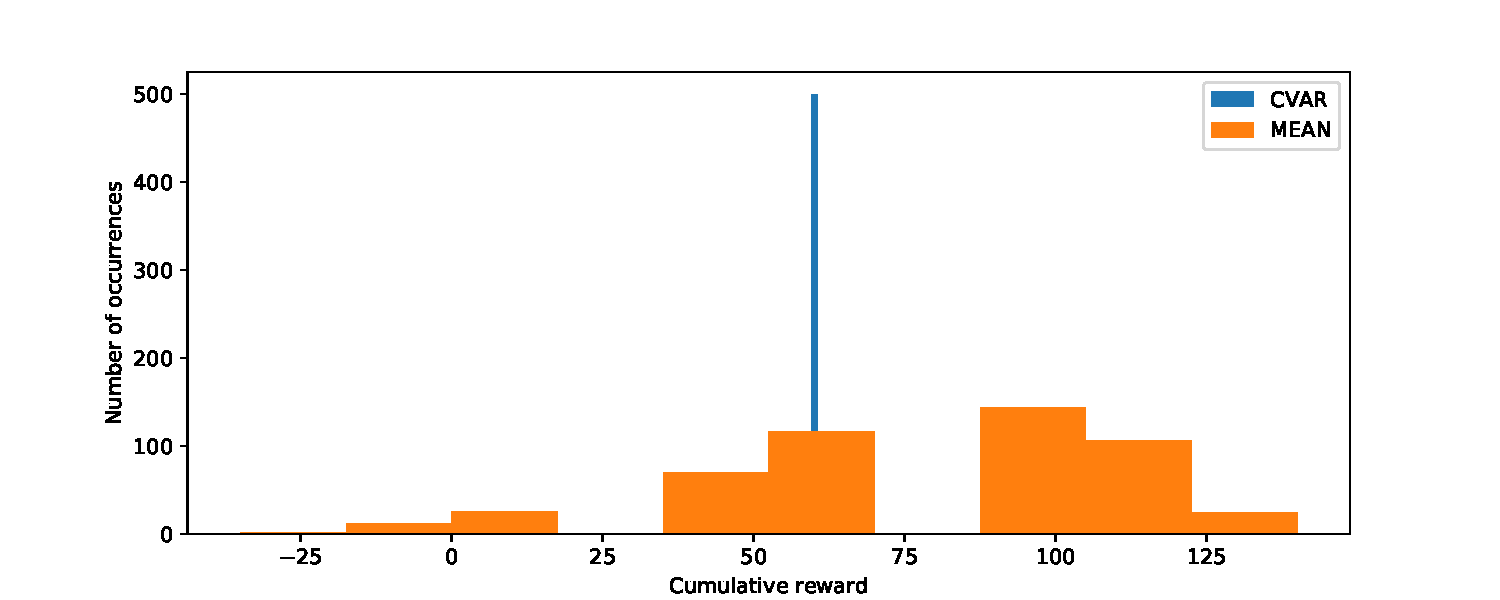
\includegraphics[width=0.8\textwidth]{images/Car/histogram_rewards1vs01.pdf}
        \caption{Comparison of cumulative rewards achieved with CVAR-DDPG  algorithms with $\alpha$= 0.2
        and $\alpha$= 1 when the probability of velocity penalization = 0.2.
        Algorithm with $\alpha$= 1 achieves a higher expected value ($\mu=20.11$) but 
        has a lower CVAR ($\text{CVaR}_{\alpha= 0.1}$=-27.12 compared to the algorithm
        with $\alpha$= 0.1, which has $\mu=0$ and $\text{CVaR}_{\alpha= 0.1}$=0.0
        5000 episodes were ran after training each algorithm. }
        \label{histogram_alpha01_vs_alpha1}
    
\end{figure}

\todo{A binomial distribution can be observed.}
\begin{figure}[ht]
        \centering
        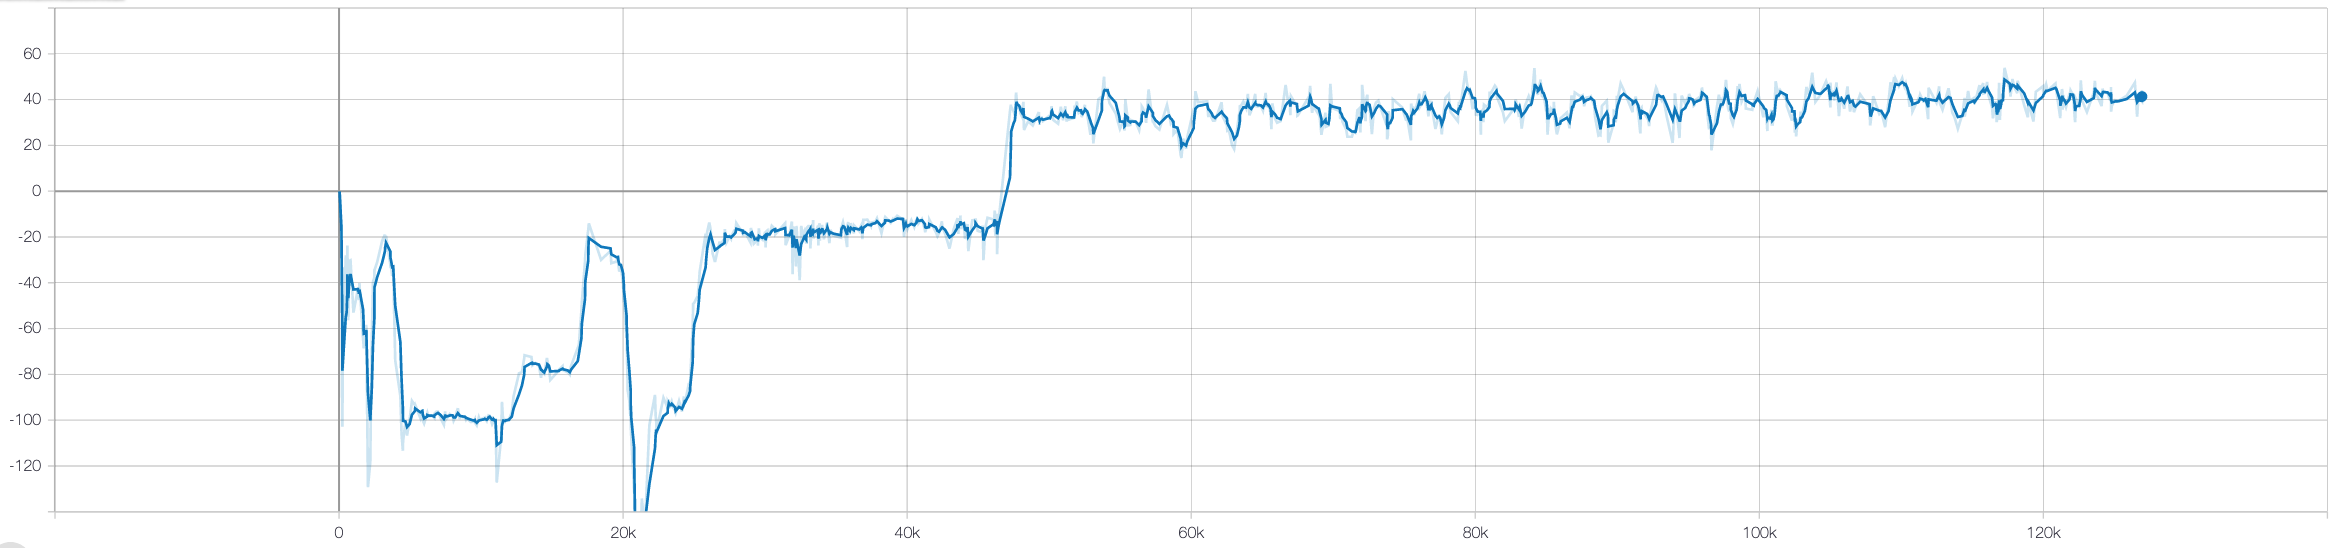
\includegraphics[width=0.8\textwidth]{images/Car/CVAR/Cvar_evol.png}
        \caption{Evolution of the sampled mean of the tail of the Cumulative Value Distribution during training epochs}
        \label{tail_CDF_EVOL}
    
\end{figure}

